\section{Experiment Records and the Supporting Response Experiment}
\label{app:empirical}

The main experiment records keep every planned combination of settings,
starting points and observation windows, including failed histories. They
also keep source-file lists, each random-number stream's state before and
after draws, and hashes of the original bytes. The complete local package
contains these records and test sources. The main theorem, which keeps
damping positive and fixed, needs neither a fit to data nor a
vanishing-damping crossover limit.

\subsection{A Reproducible Calculation of Certified Kernel Bounds}\label{app:certificate}
For the numerical smooth example, the optimizer constants are exact
dyadic numbers, meaning rational numbers with power-of-two denominators:
\[
 \alpha=\lambda=\frac{3602879701896397}{36028797018963968},\quad
 \beta=\frac{3602879701896397}{18014398509481984},\quad
 \epsilon=\frac{1080863910568919}{36028797018963968}.
\]
The displayed decimal labels $.1,.2,.03$ abbreviate these binary64 values.
The SGD controls evaluated at exact decimal fractions are a separate
nominal reference.
The general existence theorem does not depend on this computer-assisted
numerical instance.

Each coordinate's noise magnitude at the optimum has $R^2\sim\operatorname{Bernoulli}(1/2)$.
Thus its square is zero or one with equal probability. For $L=14$,
$J=8$, and $b\in\{0,1\}^L$, define
\[
 D_j(b,r)^2=\sum_{\substack{0\leq k<L\\k\ne j}}d_kb_k+d_jr^2,
 \qquad c_j=d_jr^2,\qquad r\in\{0,1\},
\]
and the finite exact expectation
\[
 S_{L,J}(r)=2^{-L}\sum_{b\in\{0,1\}^L}\sum_{j=0}^{J-1}w_j
 \left[\frac1{D_j(b,r)+\epsilon}
       -\frac{c_j}{D_j(b,r)(D_j(b,r)+\epsilon)^2}\right].
\]
For $r=0$, the bracket is defined as $1/(D_j+\epsilon)$, including
at $D_j=0$. Each own-time bit $b_j$ is removed before substituting $r$;
the two copies of each remaining bit pattern in the $2^{14}$ enumeration
correctly average over the other $13$ bits. They do not condition on a
bit that should have been removed.
If $\beta=p/q$, every prefix energy uses the exact common integer denominator
$q^L$, with numerator weights $(q-p)p^kq^{L-k-1}$.

For $D\geq\sqrt c$, let
$k_c(D)=1/(D+\epsilon)-c/[D(D+\epsilon)^2]$ with the same zero convention.
Direct differentiation and $c\leq D^2$ give
$|k_c'(D)|\leq4/\epsilon^2$. The omitted squared RMS history is at most
$\beta^L$, hence its RMS displacement is at most $\sqrt{\beta^L}$.
Since the weights sum to one and the complete omitted numerator tail is
$\alpha^J$, the uniform deterministic enclosure is
\begin{equation}\label{eq:kernel-certificate-error}
 |\Psi(r)-S_{L,J}(r)|
 \leq\frac{4\sqrt{\beta^L}}{\epsilon^2}+\frac{\alpha^J}{\epsilon}
 <.056889222222223.
\end{equation}
This error comes from omitting old history terms; it is a deterministic
bound, not sampling uncertainty.

We bound the finite sums using 48-significant-digit Decimal arithmetic,
rounding every interval outward so that it contains the true value. Exact rational inputs are divided with floor/ceiling rounding;
correctly rounded nearest square roots are enclosed by their adjacent
representable values. Subsequent interval operations round outward. The
resulting finite intervals, rounded further outward here, are
\begin{align*}
 S_{14,8}(0)&\in[5.7600901401318146058334218,
                    5.7600901401318146058334219],\\
 S_{14,8}(1)&\in[.1837568600091745741532676,
                    .1837568600091745741532677].
\end{align*}
The unrounded intervals plus \eqref{eq:kernel-certificate-error} give the
kernel bounds in Section~\ref{sec:matrix-experiment}. Carrying these
bounds through the linear formulas gives the four field-eigenvalue
intervals. The kernel does not depend on the Hessian. The calculation
script is
\path{experiments/q2_matrix_susceptibility_certificate_20261117.py},
source SHA256
\path{eda13382f7e4798d1e865bf3894c4875ec890efba2ae808fd3acad072f409a99},
with full output in
\path{results/q2_matrix_susceptibility_certificate_20261117.json}.
The resulting bounds for the matrix example are recorded separately in
\path{results/q2_conditioned_matrix_fixture_20261117.json}.
These finite formulas, error bounds and outward-rounding operations make
the numerical example checkable. No mathematical claim relies on an
unspecified fit to data.

\begin{figure}[htbp]
\centering
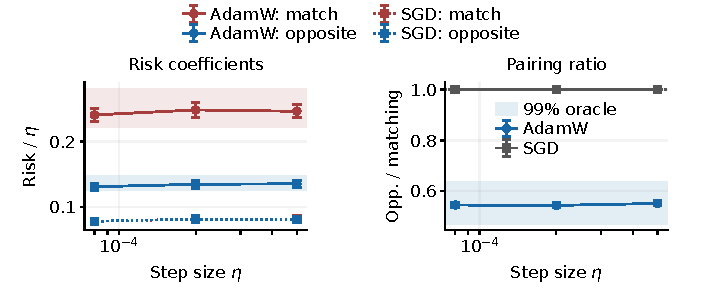
\includegraphics[width=\linewidth]{figures/scalar_couplings.pdf}
\caption{Supporting scalar classification experiment: all three fixed
steps in the predeclared zero-start final-window display. Left: normalized
population risks for both optimizers and both rank couplings. Right:
opposite/equal-rank risk ratios. Empirical error bars are approximate
pointwise 95\% intervals. Shading represents separately computed independent
asymptotic oracle enclosures (joint 99\% oracle event), excluding unknown
finite-step errors. The two uncertainty statements are not a combined
coverage guarantee. Both AdamW arms have higher absolute risk than SGD. Plotting code was developed with OpenAI Codex; displayed quantities are derived from recorded numerical outputs.}
\label{fig:scalar-couplings}
\end{figure}

\paragraph{Earlier checks of absolute predictions.}
The original rare-pulse grid used $n=256,320,384$, aligned phase $.5$,
four damping ratios and 256 paired replicas at starts $0,\pm8r$.
Only 15 of its 108 approximate simultaneous moment bands intersected the
independent leading oracle intervals; 12 intersected a separately frozen
diffusion-only proxy. These are intersections between separately constructed bands,
not a combined confidence test. The new $n=448$ absolute holdout used a
different, shorter fixed observation clock. Its simultaneous bands intersect
both the leading and first-response functional intervals in every one of
36 correlated features, despite all point estimates lying in the wider
response intervals. Neither study bounds the error at finite rates or the time required to
reach stationarity. These discrepancies remain unchanged.

\paragraph{A planned comparison that cancels the shared leading term.}
The new supporting experiment keeps the original disjoint B gradient
distribution with
$q=1/64$, pulse amplitude $.25$, $\alpha=.9$, $\beta=.95$ and its
unchanged quartic repair coefficient $1.5438843199133034\cdot10^{-5}$.
Compare decays $\lambda_{\rm lo}=.1$ and $\lambda_{\rm hi}=52.1$ at
$c=\epsilon/r=30$. The two aligned rates have
$r=\rho^{n+1/2}$, $\eta=r^{1+\gamma}$,
$\gamma=\log(63/64)/\log\rho$, $n=384,448$.
Both rates and decays use exactly the same critical-clock windows
$8.25{:}.25{:}16$, $16.25{:}.25{:}24$, $24.25{:}.25{:}32$,
256 replica columns and the three starts $0,\pm8r$.

Subtracting the companion first stationary-response expansions cancels
both the common leading moment and its regular-field coefficient. For
$\delta=r^{1-\gamma}$, the fixed functional prediction is
\[
 \E_{\rm hi}(u/r)^2-\E_{\rm lo}(u/r)^2
   =-\delta\frac{52}{D_0}\operatorname{Var}_{\pi_{\theta,c}}(Y^2)
          +o(\delta).
\]
The limiting law and $D_0$ were evaluated from the earlier independent
oracle data, with directed interval propagation before this new generator.
The theorem for this response and its expanded proof remain in the
companion manuscript. No core proof here uses them as a lemma.
The 98\% joint oracle statement covers only this fixed asymptotic
functional, excluding its unknown finite-rate remainder and equilibration.

All trajectories completed. The 18 main paired comparisons include both
rates and every starting point and window. Their simultaneous upper
endpoints are all below zero. The planned display for the zero start
and final window is shown in Table~\ref{tab:decay-response}:
\begin{table}[htbp]
\caption{Prospective Paired-Decay Response at the Final Window}\label{tab:decay-response}
\centering

\small
\begin{tabular}{cccc}
\toprule
$n$ & \shortstack{High minus low\\second moment} & \shortstack{Approx. simultaneous\\95\% interval} & Contrast/$\delta$\\
\midrule
384 & $-.02466308$ & $[-.02658672,-.02273944]$ & $-1.108985$\\
448 & $-.01368078$ & $[-.01484302,-.01251854]$ & $-1.159072$\\
\bottomrule
\end{tabular}
\end{table}
The displayed simultaneous endpoints are rounded outward. The common
independent functional interval for contrast/$\delta$ is
$[-1.406947,-.885859]$, also rounded outward. The normalized simultaneous
intervals are $[-1.195482,-1.022487]$ and $[-1.257540,-1.060604]$,
respectively. All predictions were fixed before the new trajectories.
Approximate bootstrap and independent functional uncertainty are separate
statements. The 18 quantities are dependent; their agreement does not provide 18
independent confirmations. Every one of the 18 complete simultaneous contrast intervals
also lies inside its independently frozen response-functional interval.
The descriptive window checks, whose intervals have no multiple-comparison
adjustment, are less uniform: six of 48 bands
exclude zero, all for positive late-minus-middle changes at the finer rate,
in both decay arms and repeated across the three starts. These are correlated
features, not six independent failures, and leave possible finite-clock drift
or Monte Carlo window fluctuations unresolved. This shows the sign of the decay response at the tested finite rates and
is compatible with the proposed correction. It neither fits an asymptotic
exponent nor bounds the remaining error.

\begin{figure}[htbp]
\centering
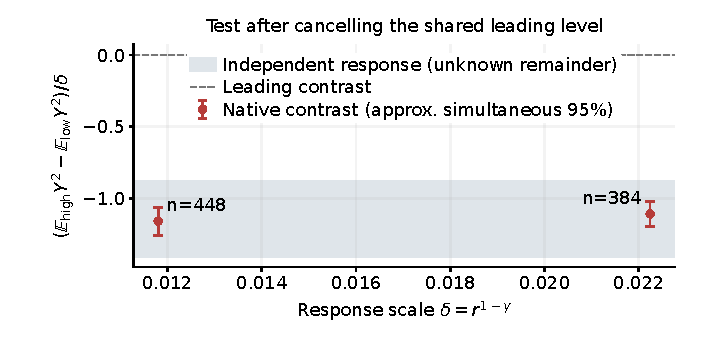
\includegraphics[width=.95\linewidth]{figures/decay_contrast.pdf}
\caption{Companion paired-decay response: the complete predeclared
zero-start final-window display at both rates, normalized by
$\delta=r^{1-\gamma}$. Red error bars are approximate simultaneous 95\%
bands from the full 18-coordinate primary family. Shading is the separately
frozen response-functional enclosure (98\% joint oracle event); its unknown
finite-rate remainder and equilibration error are excluded. The dashed zero
line is the cancelled leading contrast. The plot fits no exponent and
does not retrospectively validate the preserved earlier absolute predictions. Plotting code was developed with OpenAI Codex; displayed quantities are derived from recorded numerical outputs.}
\label{fig:decay-contrast}
\end{figure}

\paragraph{Scope of the main matrix experiment.}
The matrix example with moderate condition number was fixed independently
of the new trajectories. Its mathematical certificate checks eigenvalue
signs for the discrete law. A separate proof shows that these signs
persist after adding a fixed smooth perturbation in every coordinate. Three step sizes, both optimizers and both copulas,
three starts and all windows remain in the final matrix consumer.
These finite observation windows must be distinguished from the theorem,
which applies asymptotically to every invariant selection. Neither the
matrix nor the pulse experiment establishes a neural-training benefit.
